\documentclass{article}
\usepackage[utf8]{inputenc}

\title{Computación Distribuida \\ Tarea 02}
\author{Olea Olvera Marco Iván \\ Arteaga Hernández Labín}
\date{}

\usepackage[top=1.5cm, bottom=1.5cm, left=2cm, right=2cm]{geometry}
\usepackage{fouriernc}
\usepackage{amssymb}
\usepackage{listings}
\lstset{
  basicstyle=\ttfamily,
  mathescape
}

\usepackage{graphicx}
\graphicspath{{./}}

\begin{document}

\maketitle

\section{}

Cada nodo tiene un identificador \textit{pid}, una variable \textit{poblacion} cuyo valor es la cantidad de pobladores en cierto diámetro, y una variable \textit{neighbors} que representa el conjunto de sus vecinos.

\begin{lstlisting}
initially do
  children $\leftarrow$ $\varnothing$
  nonChildren $\leftarrow$ $\varnothing$
  parent $\leftarrow$ $\bot$
  if pid = root then
    parent $\leftarrow$ root
    send init to all neighbors
    
upon receiving init from q do
  if parent = $\bot$ then
    parent $\leftarrow$ q
    send init to all neighbors
  else
    send nack to q
    
upon receiving nack from q do
  add q to nonChildren
  
as soon as children U nonChildren = neighbors do
  if pid = root then
    return poblacion    // Termina el algoritmo.
  else
    pob_hijo $\leftarrow$ poblacion
    send ack(pob_hijo) to parent
    
upon receiving ack(pob_hijo) from q do
  poblacion $\leftarrow$ poblacion + pob_hijo
  add q to children
\end{lstlisting} \newpage

\section{}

El algoritmo depende de la velocidad de los mensajes GO(). Es decir, el padre de un nodo depende de cuál de sus vecinos le envía primero el mensaje GO().

Por ejemplo, supongamos la siguiente red (izquierda) con raíz $A$.

\begin{figure}[h]
    \centering
    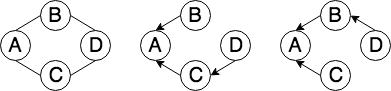
\includegraphics[scale=0.7]{fig.png}
\end{figure}

$A$ le mandará el mensaje GO() a $B$ y $C$, estos asignarán a $A$ como su padre, y cada uno de estos, entre otras cosas, le mandarán GO() a $D$, pero no podemos saber cuál de estos dos mensajes llegarán primero a $D$.

Si a $D$ le llega primero el mensaje GO() de $C$, resulta el árbol de en medio. De lo contrario, resulta el árbol de la derecha.

\section{}

Como el algoritmo envía a lo más $|V||E|$ mensajes, toma tiempo $|V| \Sigma_{e \in E} w(e)$, donde $w(e)$ es el peso de la arista $e$.

\section{}

\subsection{}
Cada nodo recibe exactamente un \textit{vis} de cada uno de sus vecinos, así que
 el algoritmo ocupa al menos $|V|$ pasos. Además, sabemos que cada arista del árbol generador resultante habrá sido usado para mandar el \textit{token} exactamente dos veces, una vez "de ida" y luego "de regreso". Como el árbol tendrá $|V| - 1$ aristas, entonces el algoritmo ocupa $|V| + 2(|V| - 1) = 3|V| - 2$ pasos. Es decir, es $O(|V|)$ en tiempo.
 
 \subsection{}
 Todos los nodos en algún momento mandaran \textit{vis} a todos sus vecinos (en la línea 5 o 18), esto es, habrán $2|E|$ mensajes \textit{vis}. Pero no todas las aristas de la gráfica se usarán para mandar \textit{token}, sólo $|V| - 1$ de ellas. Entonces habrán $2(|V| - 1)$ \textit{tokens}, lo cual da un total de $2|E| + 2(|V| - 1) = 2(|E| + |V| - 1)$ mensajes, y como $|V| - 1 \leq |E|$ (si no, sería disconexa), la complejidad es $O(|E|)$ mensajes.
 
\end{document}
